%Color Chapter: Ph.D. thesis, J.A. Brindle last modified 22.01.14
%Read Levinson 2000
%change subject to consultant 
\chapter{Color}
\label{sec:COL-chap}

\section{Introduction}
\label{intro}

This chapter investigates  color terms. First it presents  an attempt to
discover the language's  \textit{basic color terms}, as  defined in
\cite{Berl69}. It addresses  the possibility of placing the language
provisionally 
within a typology of basic color terms despite some methodological
deficiencies.   For the allotment of Chakali within the typology to be achieved,
one needs to confirm a number of basic color terms. The question of how one
achieves the assignment of expressions to basic color terms is explored. 

Since it is widely accepted that most of the languages of Africa typically
contain few color terms, the hypothesis is  that Chakali is no more complex or
simple in that domain than the other languages of the Northern Ghana
\citep{Nade05}. Thus the null hypothesis is that Chakali  has at least three
color terms and a multitude of other expressions to convey instances of color.  


%Secondly the section introduces descriptive and connotative
%usage of the color terms discovered.  



%As an exercise,  an algorithm is provided which extract the basic color term
%from the naming data. 



 
\section{Basic Color Terms: an overview}
\label{sec:basiccolor}

The linguistics and psychology of basic color terms was originally investigated
by researchers working in a  language-relativistic framework (\cite{Brow54,
Conk55}
among others). The notion of basicness was seen as an internal structure of a
color system in which a limited number of color terms reflected perceptual
opposition. In the early sixties, a project directed by Brent Berlin, Paul Kay
and William Merrifield and funded by the National Science Foundation and
University
of Berkeley undertook a cross-linguistic study of color terms. The
hypotheses advanced were first available in \cite{Berl69}.\footnote{Also of
great value are the subsequent publications on the topic  from each individual
(either jointly or not) until today. The reader is refered to the bibliography
in
\cite{Berl69} for studies on the topic previous to 1969.  An insightful
history of the topic is found  in
\cite{Saun00}.} The original project
 defined basic color terms, like its predecessors, as an attempt to identify the
smallest set
of simple and salient words that characterize the color of objects. However unlike its predecessors  the two
major conclusions of the research demonstrate the universality and evolutionary
nature of    basic color terms. 

First, they showed that  unrelated languages tend to contain the atoms necessary
to promote a set of color categories, therefore disproving the
``Sapir-Whorf''-hypothesis, which states that cultural relativism 
demonstrates a
relationship between culture and language. They observed that ``color words
translate too easily among various pairs of unrelated languages for the extreme
linguistic relativity thesis to be valid'' \cite[2]{Berl69}. Their second
conclusion is that languages ought to develop in a predictable way. They assert
that there is a partially fixed evolutionary
progression according to which languages gain color terms over time. After
compiling 98 languages, the authors showed that there is an  inventory of eleven
basic color categories (i.e. white, black, red, green, yellow, blue, brown,
purple, pink, orange and grey) and that they are organized in a
hierarchy.\footnote{The compilation was gathered into two `steps'; in the first
one the data of 20 languages was collected with the help of native speakers, and
in the second step the data was taken from language documentation (i.e.
descriptive grammars, ethnographies, dictionaries) and personal communication.} 
The claim is that  if a language has fewer than eleven categories, there are
restrictions regarding possible systems. The authors identify twenty-two {\it
types} of language out of a logically possible 2048 combinations of the eleven
basic color categories (i.e. $2^{11}$).  They list the following restrictions:

%Cultural relativism was also refuted
% in \cite{Kay05b} and is not relevant for the present discussion.

\begin{enumerate}\addtolength{\itemsep}{-0.5\baselineskip}
\item All languages contain terms for white and black.
 \item If a language contains three terms, then it contains a term for red.
\item If a language contains four terms, then it contains a term for either
green or yellow (but not both).
\item If a language contains five terms, then it contains terms for green and
yellow.
\item If a language contains six terms, then it contains a term for blue.
\item If a language contains seven terms, then it contains a term for brown.
\item If a language contains eight or more terms, then it contains a term for
purple, pink, orange, grey, or some combination of these.
\end{enumerate}


 %and that each language is semantically non-arbitrarily
%relative to every other language, since they all (in their data set) follow the
%implications

According to the authors, what is important to understand in those implications
is that they reflect chronological order interpreted as a sequence of
evolutionary stages.\footnote{Scholars I have discussed with agree that this
claim is exceedingly simplistic. It has not been demonstrated that, for example,
a language with a system of six basic color terms derives historically from a
language that had five basic color terms (Prof. Giorgio Banti p.c.).
Theoretically one can also envisage that a more complex system gets simplified
during its history. \cite{Kris80} demonstrates that the evolution of color
systems is not always linear since regression is attested in some dialects of
Italian.} The  original evolutionary schemata \cite[4]{Berl69}  is reproduced in
(\ref{ex:schemata}). It was first revised in \citet[260-261]{Kay75} and
subsequently in other publications. The revisions concern mainly the first
stages. The schemata in \cite{Kay97} is discussed in section \ref{sec:prel}.


\begin{exe}
  \ex\label{ex:schemata}
For distinct color categories $(a,b)$, the expression $a< b$ signifies that $a$
is present in every language in which $b$ is present and also in some language
in which $b$ is not present.


%\begin{figure}[h!]
  \centering
$ \left[
  \begin{array}{ l  }
   white  \\
   black
  \end{array} \right]
  < [red] < \left[
  \begin{array}{ l  }
  yellow  \\
   green
  \end{array} \right] < [blue] < [brown] < \left[
  \begin{array}{l }
  purple\\
 pink\\
 orange\\
 grey
  \end{array} \right]
$



%\end{figure}
\end{exe}


In their typology a language type is a
particular evolutionary  stage. The number and the members of the set of basic
color terms
define the type.   Consequently a language which presents a lexicon of only two
terms (i.e. only
black/dark and white/bright) must reflect an instance of  {\it type 1/stage I}
language 
and if the language changes and lexicalizes another color term, that term must
be red (thus the language becomes a \textit{type 2/stage II} language, see figure
\ref{fig:berlkay3}).  Given  a language with a term for `red', there are only
two possible evolutionary paths: either yellow (\textit{type 3/stage IIIb})  or
green (\textit{type 4/stage IIIa}) could be  basic in the next stage. 

\begin{figure}
  \centering
   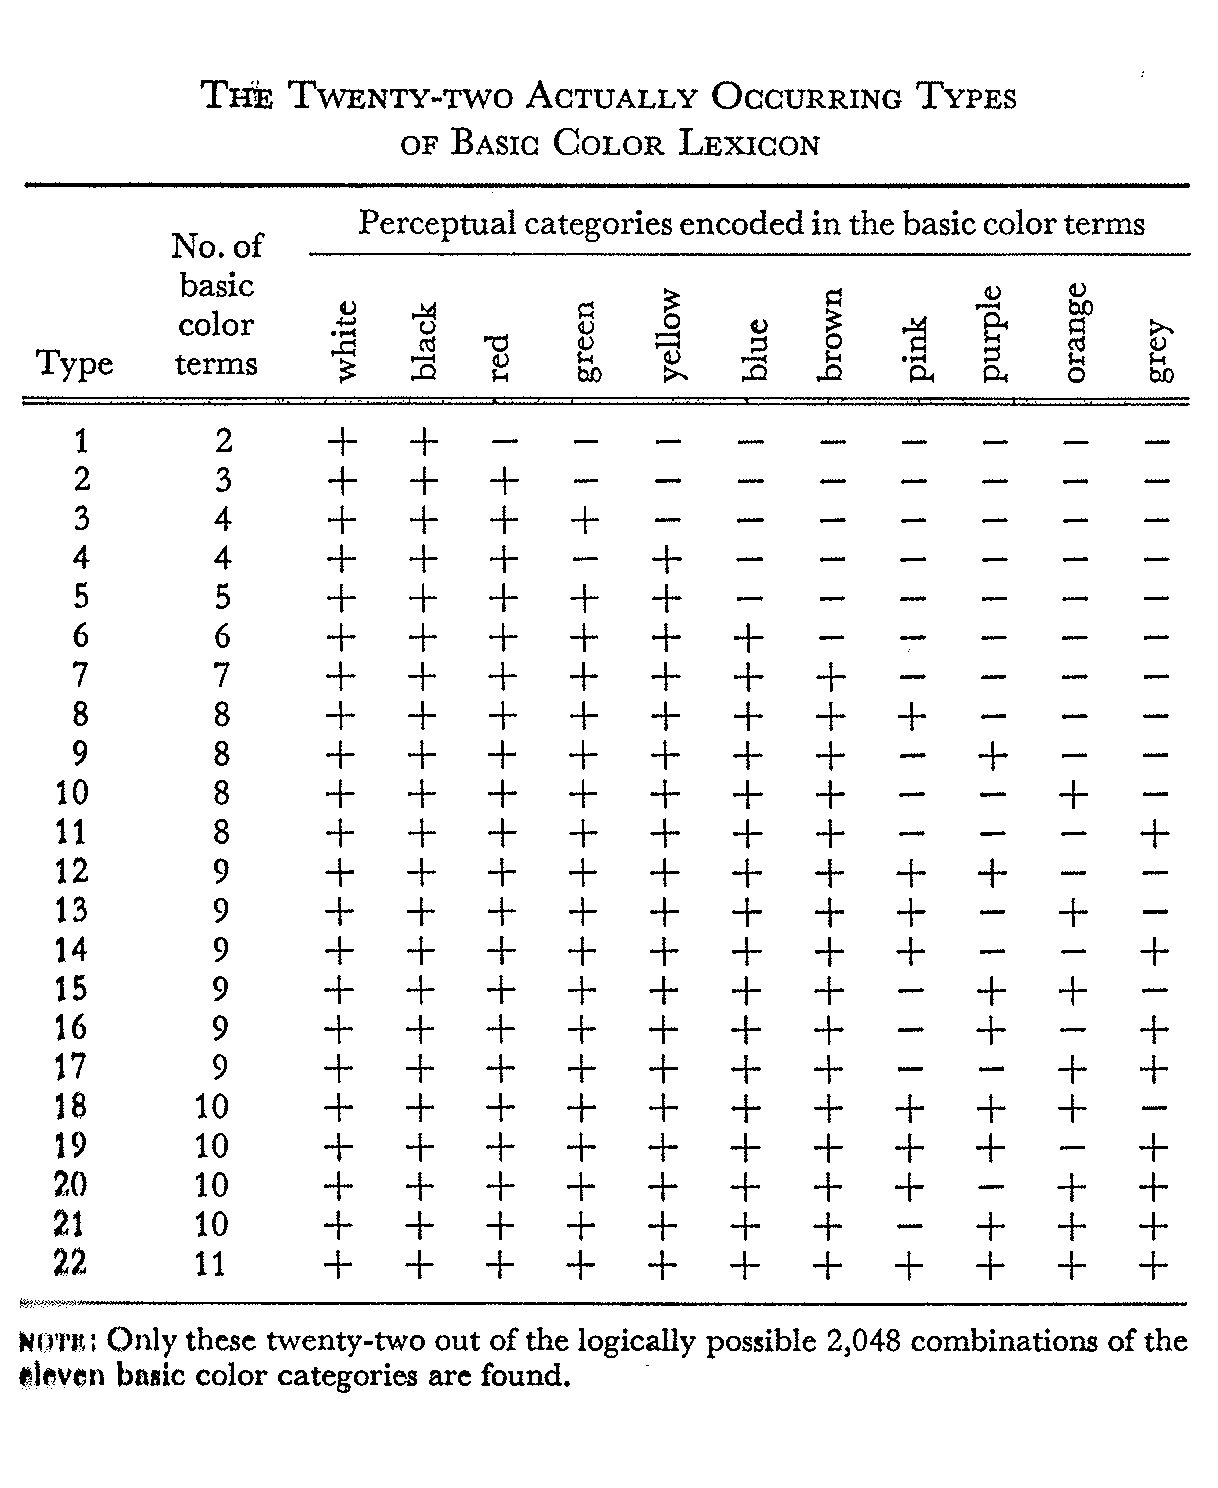
\includegraphics[width=5in]{Graphic/Pictures/BerlKay3.jpg}
  \caption{\citealp[3]{Berl69}}
  \label{fig:berlkay3}
\end{figure}

\subsection{Recognized Methods}
\label{sec:recmeth}

Three methods used  to identify the basic color terms of a language are
presented: the list task, the tile naming task and the focal task. The reader is
referred to \cite{Lenn61, Lant64, Lenn67, Davi94, Smit93, Davi98, Borg99} for
other approaches.  The methods presented below provide the researcher with
different kinds of information. The choice of the method depends on what she/he
wants to test and measure. The assessment of a language's basic color terms
is usually based on the combination of several methods \citep[see][]{Davi92,
Corb97}. There are standards all methods seem to agree upon: the average number
of consultants should at least be between  twenty to thirty for the
results to be significant. Moreover an experiment is ideally carried out  in a
monolingual setting and at the location where the language is
spoken.


\subsubsection{List task}
\label{sec:listtask}

The list task does not limit its scope to color terms: other domains like smell,
temperature, etc. are also investigated using this test. It essentially requires
that consultants  answer the question ``Please list all Xs that you know'' 
where
X is replaced by the domain examined. The responses can be either oral or
written. The list task's results are calculated in the following manner. First
one establishes a  frequency parameter by  getting rid of terms that are
used by few speakers since those terms are considered  accidental/occasional.
This is an arbitrary criterion and is motivated by the fact that low frequency
terms are not expected to be in active use in the language, so cannot be
considered as basic. Second the mean point parameter calculates the mean
point of a term for each consultant using the  list containing that term.
According
to \citet[265]{Sutr01}, it is generally accepted that ``there is a good
correlation between the frequency and the mean rank of a term (i.e. the most
frequent terms are named first and the terms that are named only by a few
consultants
are named last)''. \citeauthor{Sutr01} proposes the integral {\it cognitive
salience index} where both the frequency and the mean parameters are combined to
define saliency. Salience ($S$) is a fraction $S=F/(N \ mP)$ ``in which the
dividend considers the frequency ($F$) with which a term is named
in the list task. The divisor $N \ mP$ considers the weight of the mean position
$mP$ in which the term is named, and $N$ is the number of consultants''. The
list
task provides the researcher with (i) the most prominent words for a given
domain for each consultant and for representative groups and (ii) the common
reference of specific words. The \textit{list task} of \cite{Davi94,
Sutr98, Sutr01} is equivalent to the \textit{free list} in \cite{Smit93} and 
\textit{Approach A} in \citet[340]{Lenn67}.


\subsubsection{Tile naming task}
\label{sec:chiptask}

The tile naming task requires  consultants to name the color presented to
them
on tiles. For the  World Color Survey, consultants are requested  to name
each
of the 320 Munsell chips, shown in a constant, random order.\footnote{``The
World Color Survey was initiated in the late 1970's to test the hypotheses
advanced in \cite{Berl69} regarding (i) the existence of universal constraints
on cross-language color naming, and (ii) the existence of a partially fixed
evolutionary progression according to which languages gain color terms over
time'' (quoted from http://www.icsi.berkeley.edu/wcs/ and accessed 01/09/08).
See http://www.icsi.berkeley.edu/wcs/images/WCS for  the original instruction
sheets (1976-78) provided to field workers.} In both the World Color Survey and
in \cite{Davi95}, the number
of consultants are set to at least twenty-five adult monolingual speakers.
From the
 tile naming task's  data, one can estimate the probability of an expression to
refer to a certain tile.  The tile task is equivalent to the \textit{Approach B}
in \citet[340]{Lenn67}. 

%which yields a variable called \textit{codability} \cite[345]{Lenn67}. We
%shall
%return to this notion in section \ref{sec:result}.
%, but can also aligned with the  \citeauthor{Sutr01}'s notion of  the saliency
%discussed in section \ref{sec:listtask}.


\subsubsection{Focal task}
\label{sec:focaltask}


For the  focal task,  consultants are asked to identify on an array (or a
palette)  of colors 
the point/region where a color term is the more appropriate.\footnote{A stimulus
array is the structured assembly of the tiles. In  \citet[5]{Berl69}, the
array is a set of ``320
color chips of forty equally spaced hues and eight degrees of brightness, all at
maximum saturation, and nine chips of neutral hue (white, black and grey)''.}
Using the focal task, the researcher gathers the best examples provided by the
consultants, then calculates the mean of those points/regions. The mean result
forms
the focus of a term.   The focal task  follows either the list task or the tile
task, or both. The reason is that in the procedure the researcher must know a
certain number of color terms to be able to ask what are the points/regions which 
  best fit the terms.


\section{Color terms in Chakali}
\label{sec:chabascolor}

The only method applied to uncover the color terms of Chakali was the tile
naming task, which is presented below. However, as a follow-up study,   a short
experiment using the focal task was carried out a year
later with a
different and smaller set of  consultants. The result of this experiment is
presented in section
\ref{sec:COL-foci}.

The tile
naming task method corresponds to selecting an  evenly
distributed set of color samples in the color space, then showing native
speakers each color and asking them what expression describes the color best.
Originally my hope was to use the method proposed in \cite{Davi95}, which
combines the list task with the tile naming task.  However one problem arose in
the application of their method: Chakali does not have an
expression equivalent to the English `color'. The closest in meaning is
probably the words {\S lalaɣasa} and {\S ʔirii}. In the proverb given in
(\ref{ex:proverb-guifow}),  the word {\S lalaɣasa} is glossed as
 `plumage',  but more generally it could mean `surface visual patterns'.

%fix thing below
\begin{exe}
 \ex\label{ex:proverb-guifow}
\gll sũ̀ṹ làlàɣàsá wàá kɪ̀ŋ kùrò\\
guinea.fowl plumage \textsc{neg}  \textsc{abl} count \\
\glt `The {\it colors} of a guinea fowl cannot be counted'
\end{exe}


When one wishes to distinguish the appearance of objects, the words
{\S ʔíríí} and {\S ʔíríŋ} -- which are etymogically Hausa --  may be used by both Chakali and Waali speakers
respectively  to mean `type',  as
(\ref{ex:type-color}) illustrates.\footnote{The Waalas used {\F ʔíríŋ} to
classify people according to tribe/clan/group as well:
\begin{exe}
\sn[]{
\gll bò ʔíríŋ lá à bìé ŋã̀?  kàmbɔ̀ŋà lá\\
{\q}  type {\foc} {\art} child {\dem}  Ashanti {\foc} \\
\glt `What tribe does this child belong to?'  `The Ashanti.'}
\end{exe}
}


\begin{exe}
\ex\label{ex:type-color}{\it Shopping for a cloth}
\gll A: bàáŋ ʔíríí ɪ̀ kàà búúrè\\
{}  {\sc q} type {\sc 2.sg} {\sc egr} want\\
\glt {} `What type do you want?' (referring to cloths)

\gll B:  ʔírīī háŋ̀ \\
{} type {\sc dem} \\
\glt  `This type'
\end{exe}

A speaker of Chakali may also use {\S síí} instead of  {\S
ʔíríí} to express `type' in the context of  
(\ref{ex:type-color}).  Both {\S ʔíríí} and {\S síí} express some notions
of
categorization of visual property, but their meaning is not equivalent to what
English `color' conveys.

%Moreover, their meaning isn't as broad as type, notice the ungrammaticality
% of baaŋ sii ɪ ka buure, one must instead say kpaŋ wɪŋ ɪ ka buure 
%Does irii has a Hausa origin?


Following the   instructions proposed in \citet[27]{Davi95} (i.e. speakers are
asked to write down as many colors as they know),  lacking the word for `color'
was problematic, and  that apart from consultants'  illiteracy. Since
the list task
is an experiment which aims at gathering a speaker's  selection of expressions
which enter into a hyponymous relationship with the expression `color', 
formulating the instruction while  lacking the word for `color' was challenging.
%rephrase, some repetitions
I attempted to prime consultants with one color and let them continue with
other colors, but the task was generally misunderstood. The speakers took 
too much time and/or used expressions which after consideration were
not related to `color'.  Each list task session became a  unique event and I
 did not see how I could consider the compilation as reliable and
comparable data. In addition I often ended up having  no control over the
instruction,
after the few lines that my assistant and I had  agreed
upon were  given.
That led
to consultants feeling uncomfortable and under pressure, as the instructions
were
sometimes  too vague. For those reasons the list task was dropped altogether.


\subsection{Procedure}
\label{sec:procedure}

The data collection was carried out solely in the village Ducie during the month
of March in 2008. The participants in an elicitation session consisted of a
consultant, an assistant, who  was a native speaker with knowledge of  a common
language with both the researcher  and the consultant, and the researcher.
Altogether twenty-six consultants,  two assistants and one researcher
participated in the experiment. The elicitation sessions took place outside
under (the shade of) the roof of an open hut, always between 10:00 and 14:00. A
typical session lasted 15 minutes.  All sessions were audio-recorded and
transcribed on site.


\subsection{Stimuli}
\label{sec:stimuli}

A tile is a 4 1/2  $\times$  6 inch color paper. Each tile was placed on a  8 
$\times$  10 inch piece of plywood covered with a grey plastic sheet at about
20 inches from the consultant's eyes.  There were 62 color papers chosen from
the
Color-Aid Corporation range. The selection was evenly distributed on the color
space.\footnote{The rationale of the selection is given in
\citet[1097]{Davi92}.}  The Color-Aid Corporation uses the Ostwald color
system \citep{Ostw39, Pacl83}. The Ostwald color system renders a color space
based on dominant wavelength, purity, and luminance, mapping the values of hue,
saturation and brightness. For the chromatic colors, the tiles used in the
experiment were assigned a distinctive value based on whether it was a full
color
(HUE), a tint (T) or a shade (S). The hue symbols are Y=yellow, O=orange, R=red,
G=green, V=violet and B=blue and their combinations (e.g
OYO=orange-yellow-orange). Tints are perceived as the degrees of whiteness with
minimal blackness perceived, while shades are the opposite. Each hue is
affected
by a degree of four tints or three shades; so a tile labelled GYG-T4 means
green-yellow-green with the highest degree of whiteness with minimal blackness
perceived. For such a tile, according to \citet[34]{Davi95}, a majority of
English speakers would name it green, but others might name the same  tile
light green,
pastel green or lime green.  The achromatic colors are represented in the 
samples by one black tile, one white tile and five greys scaling between black
and white. The reason why 62 tiles were used as compared to 65 in \cite{Davi95}
is that the tiles RO-hue, RO-T3 and RO-S3 were destroyed at the field. On one
hand
this situation creates a drawback for future comparative studies since most
recent studies on basic color terms use the tile naming task as described in
\cite{Davi95}. On the other hand,  considering the purpose of the present
study, this inconvenience does not affect the result.
 

\subsection{Consultants}
\label{sec:consultants}

Twenty-six consultants performed  the task: thirteen individuals of both sexes.
Among them, two were twelve-year-old school children, one male and one female.
The reason the two school children were included in the experiment arose from my
 suspicion that some years of formal education might affect their lexicon. That
was not confirmed as  will be shown below. The selection of the twenty-four
adult consultants reflects a distribution of the village's sections. Table
\ref{tabːconsultant-info} provides information on each consultant in this order:
a four letter identification code, sex, age, section of Ducie where she/he
lives, mother's origin and father's origin.\footnote{The age assigned to each
individual is an approximation based on the age of the assistants, who both knew
their age. For a Chakali, it is more practical to know whether you are younger
or older than someone else, than to know your absolute age. Since both
assistants knew their own absolute age, we were able to estimate the age of
others.} If an individual had a parent from a non-E3 village (see section
\ref{sec:SOC-overall-vitality}),  she/he was asked about her/his background.
Additional criteria for
participation were that (i) the consultant had not spent more than one year
outside the village in a non-E3 village, (ii) at least one of his/her parents
was born and raised in an E3 village,  and (iii) the consultant had never
attended school or had dropped out before primary 6.

\begin{table}[h]
\centering
\caption{Naming task: information on consultants 
\label{tabːconsultant-info}}
\begin{Itabular}{llllll}

\Hline
I.D. & sex & age & Ducie's section & orig. mother & orig. father\\
\hline

AWAI  & f & 28 & Kuorobanɪɪ & Ducie & Ducie \\ 
ADJA  & f & 40 & Paŋbanɪɪ & Ducie & Chagu  \\ 
AMAM  & f & 25 & Paŋbanɪɪ & Ducie & Kpaye \\ 
HAKU & f & 35 & Kuorobanɪɪ & Gbungwale & Ducie \\ 
ADII  & f & 20 & Kuorobanɪɪ & Gbungwale & Ducie \\ 
AKUY  & f & 22 & Paŋbanɪɪ & Motigu & Motigu  \\ 
TANI  & f & 23 & Paŋbanɪɪ & Ducie & Ducie \\ 
WOSA  & f & 32 & Paŋbanɪɪ & Bawina & Ducie  \\ 
MAMA & f & 29 & Lobanɪɪ & Belezing & Katua  \\ 
GONG  & f & 50 & Lobanɪɪ & Ducie & Ducie  \\ 
AWAA  & f & 45 & Ziŋbanɪɪ & Katua & Katua \\ 
ADZU  & f & 26 & Lobanɪɪ & Gurumbele & Gbungwale  \\ 
MANK  & m & 30 & Kuorobanɪɪ & Ducie & Ducie \\ 
DOGA  & m & 42 & Kuorobanɪɪ & Ducie & Ducie \\ 
BAKW  & m & 45 & Ziŋbanɪɪ & Gurumbele & Ducie  \\ 
ZIEN  & m & 45 & Lobanɪɪ & Ducie & Ducie \\ 
WISA  & m & 40 & Lobanɪɪ & Gbungwale & Ducie  \\ 
DINL  & m & 30 & Ziŋbanɪɪ & Motigu & Ducie  \\ 
KALA & m & 40 & Kuorobanɪɪ & Ducie & Ducie \\ 
BUOL  & m & 37 & Kuorobanɪɪ & Ducie & Ducie \\ 
ISIS  & m & 43 & Kuorobanɪɪ & Ducie & Ducie  \\ 
MANA  & m & 35 & Kuorobanɪɪ & Ducie & Ducie  \\ 
ABLE  & m & 26 & Paŋbanɪɪ & Ducie & Ducie  \\ 
KALS   & m & 37 & Paŋbanɪɪ & Gurumbele & Ducie \\ 
MALE & f & 12 & Kuorobanɪɪ & Gbungwale & Ducie  \\ 
AZAK  & m & 11 & Lobanɪɪ & Katua & Ducie  \\ 
\Hline
\end{Itabular}

\end{table}
%Where is Kpaje? see AMAM
%TABLE 

\subsection{Instruction}
\label{sec:instruction}

The instructions were given in Chakali by  one of the assistants. The
consultant was informed of the approximate number of tiles to identify and the
amount of time it might take. If they could not respond, they  simply had to
say {\S n̩ wa zɪma} `I don't know'. We made explicit that there was no time
constraint but  consultants rarely spent more than 5 seconds on a tile.
Again, given that Chakali do not have a word for `color', I decided to prime
the consultants with a color instance which I knew was a color term
before starting the task.\footnote{A similar experiment was carried out a year
earlier \citep{Brin08a}. None of the twenty-six consultants participated in the
previous experiment.} That allowed us to keep the instruction to a minimum. 
Thus each consultant was presented with an illustrative scenario where the
assistant placed the tile  BLACK, WHITE or R-HUE on the board and I, the researcher, 
answered `{\S abummo}',  `{\S apʊmma}' or   `{\S asɪama}'. The tile choice for
each illustrative scenario  was of course selected at random.

\begin{table}
\centering
\caption{Naming Task. Distribution of responses across 62 tiles
\label{tab:distribu}}
\renewcommand{\arraystretch}{0.8}
\begin{Itabular}{lllrllrlll}

\Hline
Code & & Terms & F. & Code  & Terms & F. & Code  & Terms & F. \\
\hline

Y & HUE & sʊsaʊ & 17 & S2 & bummo & 10 &  &  &  \\ 
 &  & sɪama & 4 &  & hɔlahɔla & 4 &  &  &  \\ 
 &  &  & \multicolumn{1}{l}{} &  &  & \multicolumn{1}{l}{} &  &  &  \\ 
YOY & HUE & sʊsaʊ & 16 & T4 & pʊmma & 10 & S2 & pʊmma & \multicolumn{1}{r}{8}
\\ 
 &  & hɔlahɔla & 5 &  & sʊsaʊ & 7 &  & sʊsaʊ & \multicolumn{1}{r}{4} \\ 
 &  &  & \multicolumn{1}{l}{} &  &  & \multicolumn{1}{l}{} &  &  &  \\ 
YO & HUE & sɪama & 13 & T3 & sʊsaʊ & 10 & S3 & bummo & \multicolumn{1}{r}{14}
\\ 
 &  & sʊsaʊ & 9 &  &  & \multicolumn{1}{l}{} &  &  &  \\ 
OYO & HUE & sɪama & 25 &  &  & \multicolumn{1}{l}{} &  &  &  \\ 
O & HUE & sɪama & 18 & S1 & sɪama & 10 & S3 & bummo & \multicolumn{1}{r}{12} \\ 
ORO & HUE & sɪama & 24 & T3 & sɪama & 11 & S3 &  pʊmma & \multicolumn{1}{r}{6}
\\ 
 %&  &  & \multicolumn{1}{l}{} &  &  & \multicolumn{1}{l}{} &  & pʊmma &
%\multicolumn{1}{r}{5} \\ 
ROR & HUE & sɪama & 24 & T3 & sɪama & 10 & S3 & bummo & \multicolumn{1}{r}{8}
\\ 
R & HUE & sɪama & 23 & T4 & sɪama & 4 & S3 & pʊmma & \multicolumn{1}{r}{7} \\ 
RVR & HUE & sɪama & 20 & S1 & sɪama & 11 & S3 & bummo & \multicolumn{1}{r}{15}
\\ 
RV & HUE & sɪama & 22 & T2 & sɪama & 13 &  &  &  \\ 
VRV & HUE & sɪama & 17 & S3 & bummo & 10 &  &  &  \\ 
V & HUE & sɪama & 5 &  &  & \multicolumn{1}{l}{} &  &  &  \\ 
VBV & HUE & bummo & 8 & T4 & pʊmma & 4 &  &  &  \\ 
BV & HUE & bummo & 11 & S2 & bummo & 7 &  &  &  \\ 
BVB & HUE & bummo & 13 & S3 & bummo & 21 &  &  &  \\ 
B & HUE & bulu & 11 & T1 & bulu & 12 &  &  &  \\ 
 &  & bummo & 10 &  & bummo & 7 &  &  &  \\ 
BGB & HUE & bummo & 12 & T3 & bulu & 7 &  &  &  \\ 
 &  & bulu & 9 &  &  & \multicolumn{1}{l}{} &  &  &  \\ 
BG & HUE & bulu & 13 & T1 & bulu & 6 & S2 & bulu & \multicolumn{1}{r}{4} \\ 
 &  & bummo & 7 &  &  & \multicolumn{1}{l}{} &  &  &  \\ 
GBG & HUE & bulu & 7 & S2 & bummo & 14 &  &  &  \\ 
 &  &  & \multicolumn{1}{l}{} &  & bulu & 5 &  &  &  \\ 
G & HUE & bummo & 6 & S3 & bummo & 12 &  &  &  \\ 
GYG & HUE & bulu & 7 & T4 & pʊmma & 7 & S1 & bummo & \multicolumn{1}{r}{4} \\ 
 &  &  & \multicolumn{1}{l}{} &  &  & \multicolumn{1}{l}{} &  & sʊɔsɛnɪɪ &
\multicolumn{1}{r}{3} \\ 
YG & HUE & sʊɔsɛnɪɪ & 3 & S3 & bummo & 13 &  &  &  \\ 
YGY & HUE & sʊsaʊ & 5 & S3 & sʊsaʊ & 7 &  &  &  \\ 
ROSE RED &  & sɪama & 22 &  &  & \multicolumn{1}{l}{} &  &  &  \\ 
SIENNA &  & sɪama & 17 &  &  & \multicolumn{1}{l}{} &  &  &  \\ 
WHITE &  & pʊmma & 25 &  &  & \multicolumn{1}{l}{} &  &  &  \\ 
GRAY1 &  & pʊmma & 20 &  &  & \multicolumn{1}{l}{} &  &  &  \\ 
GRAY2 &  & pʊmma & 19 &  &  & \multicolumn{1}{l}{} &  &  &  \\ 
GRAY4 &  & pʊmma & 9 &  &  & \multicolumn{1}{l}{} &  &  &  \\ 
GRAY6 &  & bummo & 7 &  &  & \multicolumn{1}{l}{} &  &  &  \\ 
GRAY8 &  & bummo & 22 &  &  & \multicolumn{1}{l}{} &  &  &  \\ 
BLACK &  & bummo & 24 &  &  & \multicolumn{1}{l}{} &  &  &  \\ 

\Hline
\end{Itabular}

\end{table}




\section{Results}
\label{sec:COL-result}


\subsection{Tile naming task}
\label{sec:chiptask}


The naming data supplied 1560 answers. This number represents the logical
possibility of 1612 (i.e. 62 tiles times 26 consultants) minus the occasions
where
a consultant did not give an answer. Thus in general consultants preferred to
utter a
term for the tile presented to them rather than to say {\S n̩ wa zima} ``I don't
know''. That might be due partly to the fact that there were no time
constraints.  The tile which gave the most difficulty to  consultants was
B-T1.
Four consultants (15\%) said that they did not know the name for the color on
the
tile. 

Table \ref{tab:distribu} displays  the Color-aid code of the tile as described
in section \ref{sec:stimuli}, the  most frequent term for each tile and their
respective frequency, which is the number of consultants who chose to use the
term to identify the tile. For some tiles, a second most frequent term  appears
under the most
frequent one. For instance, for the  symbol Y (i.e. yellow) at the top of
table \ref{tab:distribu}, the two tiles (Y-) HUE and (Y-) S2 are displayed. The
tile  Y-HUE was described as {\S sʊsaʊ} by 17 consultants and as  {\S sɪama} by
4
consultants. For the tile Y-S2, 10 consultants described it as {\S bummo} and 4
consultants as {\S hɔlahɔla}. The overall result is that  the terms {\S bummo},
{\S pʊmma} and {\S
sɪama}  spread over the distribution of responses in great majority.   To cover
the whole color space, the three terms put together account for 75\% (47/62) of
the expressions with the highest level of agreement. 


Table \ref{tab:consen-tile} displays the ten highest and lowest score for
\textit{codability}, which is a measure of how well speakers
agree in giving a name to a stimulus \citep[351]{Lenn67}.  This measure is
somehow 
equivalent to the psychological saliency criterion of  \citet[6
(iv-(2))]{Berl69}, which is  introduced in section
\ref{sec:definitionBCT}. The table shows that the highest scores of codability
relate the terms
{\S bummo}, {\S pʊmma} and {\S sɪama} to achromatic tiles, tiles with high level
of red saturation and BVB-S3. The lowest codability reveals
the upper limit of name/tile disagreement. It can also reveal that the mapping
name/tile was problematic for  consultants. Those cases reflect that 
consultants do not have a convention to name the color perceived on the tile.
For
example the tile YG-HUE was named {\S sʊɔsɛnɪɪ} by three consultants, the rest
of
the responses (i.e. 23) were all different from one another.


\begin{table}[!h]
\centering
\caption{Ten highest and lowest score of codability for a tile
\label{tab:consen-tile} }
\renewcommand{\arraystretch}{1}
 \begin{tabular}{lll|lll}
  
\Hline

Highest &&& Lowest &&\\

\hline
OYO-HUE	&	sɪama-25 &	96\% & YG-HUE	& sʊɔsɛnɪɪ-3	& 	12\% \\
WHITE	&	pʊmma-25 &	96\% & GYG-S1	& bummo-4	& 	15\% \\
BLACK	&	bummo-24 &	92\% & BG-S2	& bulu-4	&	15\% \\
ORO-HUE	&	sɪama-24 &	92\% & R-T4	& sɪama-4	&	15\% \\
ROR-HUE	&	sɪama-24 &	92\% & VBV-T4	& pʊmma-4	&	15\% \\
R-HUE	&	sɪama-23 &	88\% & YGY-HUE	& sɪsau-5	&	19\% \\
GRAY8	&	bummo-22 &	85\% & V-HUE	& sɪama-5	&	19\% \\
RV-HUE	&	sɪama-22 &	85\% & ORO-S3	& pʊmma-5	&	19\% \\
BVB-S3	&	bummo-21 &	81\% & BG-T1	& bulu-6	&	23\% \\
RVR-HUE	&	sɪama-20 &	77\% & G-HUE	& bummo-6	&	23\% \\
GRAY1	&	pʊmma-20 &	77\% &&&\\
\Hline

 \end{tabular} 

\end{table} 


On average a number of 12.5 consultants (46\%) agreed on a name for a tile and
an average of 12.9 different expressions per speaker were given to capture the
62 tiles. There is a slight difference between men and women: men gave an
average of 14 expressions to cover 62 tiles while the women gave 11.9. This
result does not support earlier studies on English \citep{Rich77, Swar78} in
which women tend to be more inclined to use a modifier with a term (e.g. light
X, dark X) or an hyponym (e.g. scarlet, marine) where men would simply use the
term, making the number of different expressions used by women larger. Even
though men provided on average more expressions than women,  I  interpret this
result as being fortuitous. 






Two school children
were included in the numbers presented so far (see table
\ref{tabːconsultant-info}). The boy AZAK gave seven
expressions to cover the 62 tiles while the girl MALE gave nine. Both of them
fall under the average number of expressions used to name the 62 tiles. They did
not
know the name of four tiles and six  tiles, respectively. Apart from MALE who
used the
expression {\S abulu} on thirteen occasions, they both used expressions the
other twenty-four consultants used. The case of {\S abulu} is treated in section
\ref{sec:yellowblue}.  Given that the 62 tiles cover the color space, it is
clear at this point that the terms {\S bummo}, {\S pʊmma}
and {\S sɪama} are employed to a much greater extent than any other terms.
 Can we call these terms \textit{basic} color terms on the basis that they are
used
 to a much greater extent than others?  Section \ref{sec:discuss} presents  a
discussion of
the naming data in light of the procedure for the determination of basic color
terms first introduced in \citet[6-7]{Berl69}. Next, we look at the result of a 
focal task.



\subsection{Focal colors}
\label{sec:COL-foci}
%what was the question asked
%This section may be moved to create a better flow
 A short experiment using the focal task was carried out a year later with five
women from Ducie and one from Gurumbele at the market in Wa. The motivation for
using the focal task was to gather the best examples, that is, to identify the
color areas (or points) to which selected Chakali color terms are associated.   
 Consultants  were given in a random order  the following nine Chakali color
terms, which at first sight, and with some brief investigation into Dagaare and
Waali, were treated as non-borrowed term: {\S bummo}, {\S pʊmma}, {\S sɪama},
{\S dʒumodʒumo}, {\S sʊsaʊ},  {\S hɔlahɔla},  {\S bʊsabʊsa},  {\S sʊɔsɛnɪɪ} and
{\S ʔileʔile}.\footnote{Two Dagaare speakers (who understand and speak Waali),
Adams Bodomo and Solomon Dansieh, could not identify a single Dagaare (or
Waali) term in  a list of 50 Chakali color terms I made for them.} To uncover
focal areas,
I  used the Color-aid color chart, which consists of 314 color chips arranged
on 4 panels.\footnote{I used the Color Chart consisting of 314 color chips
(0.5$\times$0.8 inch) distributed on 4 cards of 8 1/2 $\times$ 11 inches (Second
edition \copyright 1989-2003 Color Aid Corp). I deliberately hid the extra hue
section of one card named {\it Chart 1} which contains 10 chips. Therefore the
array contained 304 colors. {\it http://www.coloraid.com/colorchart.aspx}} Table
\ref{COL-focal-result} presents the result. 



\begin{table}[htbp]
\centering
\caption[Responses to the focal task]{Responses to the focal task with six
women from Ducie (Dw) and  Gurumbele (Gw) \label{COL-focal-result}}
\begin{Itabular}{l|llllll}
\Hline
 & Dw-1 & Dw-2 & Gw-1 & Dw-3 & Dw-4 & Dw-5 \\
\hline

bummo & Black (1) & Black (1) & Black (1) & Black (1) & Black (1) & Black (1) \\
pʊmma & White (10) & White (10) & V-LP & White (10) & White (10) & B-LP \\ 
sɪama & Rw-Hue & Rw-Hue & Rw-Hue & Rw-Hue & Rw-Hue & R-T1 \\ 
sʊɔsɛnɪɪ & YG-S1 & Ygc-Hue & G-S1 & G-S1 & G-T3 & G-S1 \\
sʊsaʊ & Y-P1-1 & Y-Hue & Y-S1 & Y-S1 & Y-Hue & Yw-T1 \\ 
hɔlahɔla & Gray (9) & Gray (4,5) & Y-P1-1 & RO-LT & YG-LP & Gray (8) \\ 
ʔileʔile & G-S1 & YG-S1 & Gray (1,5) & YGc-Hue & RV-LT & YG-S3 \\ 
dʒumodʒumo & RO-S3 & M-P3-1 & BG-LP & BV-T2 & Ygw-P3-2 & C-T3 \\
bʊsabʊsa & YG-LT & Bw-T4 & Gray (5) & O-P3-3 & Gray (4,5) & C-LT \\

\Hline
\end{Itabular}
 

\end{table}

The focal task reveals the following tri-partition. The first concerns the basic
red-white-black  whose respective identification generally points to the same
areas: (i) {\S bummo} is assigned a single chip by everyone, (ii) apart from 
V-LP and B-LP, which are very light pastel violet and blue respectively,
everyone assigns a single white chip to  {\S  pʊmma}, and (iii) for the most
part, Rw-Hue is the chip assigned to {\S sɪama}. Secondly, {\S 
sʊɔsɛnɪɪ} and {\S sʊsaʊ} are associated with  a wide range of chips, but always
with greenish ones in the case of {\S 
sʊɔsɛnɪɪ},  and yellowish ones in the case of {\S sʊsaʊ} (i.e. G and Y in
table \ref{COL-focal-result}). Thirdly, with {\S
dʒumodʒumo},  {\S hɔlahɔla},  {\S bʊsabʊsa}  and {\S ʔileʔile},  consultants
identify a wide range of chips for each color term and these chips   cannot
reliably be ascribed to a color space familiar to us. 

\section{Discussion}
\label{sec:discuss}

In this section,  the 
linguistic strategies available in building an expression referring to a color
on a tile are presented.  Then the question of how one decides whether a term is
basic or not
is addressed.


\subsection{Terms variations}
\label{sec:termvari}

The structural properties of color expressions in a particular language is often
used to categorise them grammatically. For example color terms in the European
{\it sprachbund} are typically treated as adjectives on distributional and
functional grounds. They modify head nouns and
 in some languages inflect depending on the noun agreement features. They are
used predicatively as in ``The new president is black'' and attributively as in
``The black president enters the room'' and in both cases the color term
functions
semantically  as a non-scalar property. 


In the naming data the great
majority of the 1560 expressions referring to the 62 tiles have the form  {\S
a-X} or {\S kɪn-X}. In section \ref{sec:GRM-qualifier} and \ref{sec:classifier}
respectively  these prefixes were described as  (i)
 affixing  on property- and state-denoting predicates, (ii) encoding a selection
of
semantic features of the referent to which the property modifies,  and (iii)  
 as  purely grammatical prefixes, the former renders a property into a
qualifier and the latter into a noun. Thus the words {\S
a-pʊmma} `white'  and  {\S kɪn-pʊmma} `white'  are syntactically qualifiers and
nouns
respectively. 
 Also
recurrent in the naming data is the focus marker {\S ra}, introduced in section
\ref{sec:GRM-foc-neg}, following the expressions {\S a-X} or {\S
kɪn-X}. The three frames are illustrated in (\ref{ex:most-frame}).

\begin{exe}
\ex\label{ex:most-frame}
\begin{xlist}
  \ex\label{ex:frame-qual} /a-X/  a-pʊmma [{\S ápʊ̀mmá}]  `white' 
 \ex\label{ex:frame-n}  /kɪn-X/ kɪn-pʊmma [{\S kɪ̀mpʊ̀mmá}]  `white (thing)'
 \ex\label{ex:frame-s}  /(kɪn|a)-X\#ra/  {\S kɪ̀mpʊ̀mmá rá} or {\S ápʊ̀mmá rá}
`It is white.'

\end{xlist}
\end{exe}


The three strategies in (\ref{ex:most-frame}) are not particular to the naming
data. A minimal utterance the meaning of which is carried by a property  must
obligatorily take one of the forms in (\ref{ex:most-frame}). As a result {\S
pʊmma} is an ungrammatical word in Chakali. Syntactically, the form in
(\ref{ex:frame-qual}) is identical to qualifiers found in noun phrases, 
(\ref{ex:frame-n}) is a noun and  (\ref{ex:frame-s}) is a sentence: they are
analysed as qualifier (Ql), noun (N) and sentence (S) respectively. Nonetheless
the core meaning carried in those three grammatical frames is `white'.
This is
how the color terms are represented in tables \ref{tab:distribu} and
\ref{tab:consen-tile}, that is stripped from their grammatical layers, if any. 

\begin{exe}
\exp{ex:most-frame}\label{ex:struc-most-frame}
\begin{xlist}
  \ex\label{ex:struc-frame-qual} [a-X_{prop}]_{Ql}
 \ex\label{ex:struc-frame-n}  [kɪn-X_{prop}]_{N}
 \ex\label{ex:struc-frame-s}  [[(kɪn|a)-X_{prop}] ra]_{S}  
\end{xlist}
\end{exe}

There are two exceptions to the tendency for a color term being used in one
of
the three frames. The first exception is that  an expression which also names an
object tends to not be prefixed by either  {\S a-X} or {\S kɪn-X}. Both
prefixes are excluded since what one refers to are not properties but things.
Examples are
the expressions referring to stock (e.g. {\S sʊɔsɛnɪɪ} `bean leaf
stock/broth'), woody plant products (e.g. {\S sʊsaʊ} `dawadawa powder',
{\S paatʃak} `leaf', {\S tʃambul} `residue of shea processing'),  ash
({\S tapulsa}), clay ({\S tʃur}), type of stone ({\S gbɛnɪɪ}), etc. However
some name-an-object expressions do occur on
occasions with {\S a-X} or {\S kɪn-X} (e.g. {\S asʊsaʊ} `dawadawa powder',
{\S abur} `dust'). 

The second exception is an expression which is  believed to not be Chakali. This
is represented by the  expressions {\S buluu} (158), {\S jelo} (11), {\S grin} 
(7) and {\S wait} (1).\footnote{In the remaining, a parenthesis following an
expression  indicates the number of times the expression was named throughout
the naming data or the color-aid code of a tile.}  Putting  aside {\S buluu} for
the moment, these expressions are not used by a significant proportion of
consultants. For example, {\S jelo} was used on eleven occasions by six
speakers and no two expressions identified the same tile. The tiles identified
as {\S jelo} are as diverse in the color space as Y-HUE, O-S1,  ROR-T3, R-T4,
V-HUE, BV-S2, GBG-HUE, G-HUE, ROSE RED and  GRAY6.  The expression {\S wait} was
used only once,  for the tile GYG-T4.  The expression {\S griin} was used for
the tiles RVR-S3, VRV-HUE, BG-HUE, GBG-HUE, GBG-S2 and GYG-HUE.  Apart from {\S
bulu}, these (ultimately) English expressions did not occur regularly. I
shall consider {\S buluu} in section \ref{sec:yellowblue}. Nevertheless,   the
focus marker  {\S ra} can follow all the exceptions given above. The naming data
contains expressions such as {\S sʊɔsɛnɪɪ ra}, {\S sʊsaʊ ra} and {\S bulu ro},
but nothing of the type *{\S (kɪn|a)sʊɔsɛnɪɪ}, *{\S (kɪn|a)paatʃak} or *{\S
(kɪn|a)jelo}.


The naming data contains expressions with internal structure deviating from the
three presented in (\ref{ex:most-frame}). In (\ref{ex:complex-mean}) all the
expressions consist of the sequences of two meaningful units and among them
either the term {\S pʊmma} or {\S bummo}. 


\begin{exe}
\ex\label{ex:complex-mean}
\begin{xlist}
  \ex\label{ex:complex-mean-1} tʃàmbùĺbúmmò
\ex\label{ex:complex-mean-2}  kɪ̀nhɔ̀làhɔ̀làbúmmò
\ex\label{ex:complex-mean-3}   kɪ̀nbúmmòhɔ̀làhɔ̀là
\ex\label{ex:complex-mean-4}  kɪ̀npʊ̀mmá mã́ã́bìé
\ex\label{ex:complex-mean-5}  kɪ̀nsʊ́sáʊ́ ápʊ̀mmá
\end{xlist}
\end{exe}


The first three expressions are treated as compounds, whereas the other two are
treated as phrases. In all cases  a  color term and either a color
term or another meaningful expression combine. Contrary to {\S pʊmma}, {\S
bummo} and {\S hɔlahɔla}, the words  {\S tʃambul} and {\S mããbie} in isolation
cannot suggest a color. In (\ref{ex:complex-mean-1}) the expression refers to
a kind of black, specifically a black which resembles the color of the substance
one
gets in separating the oil and the water while boiling the oil of shea nuts. The
expression
{\S tʃambulbummo} is considered an endocentric compound since the meaning of the
 noun as a whole is a variant of the meaning of {\S bummo}.  The remaining
 expressions in (\ref{ex:complex-mean}) contain the prefix {\S kɪn-} which was
said to be a noun-forming grammatical affix. The examples in
(\ref{ex:complex-mean-2}) and (\ref{ex:complex-mean-3})  differ only  with
respect
to linear order. They refer to a type of  {\S bummo} and {\S hɔlahɔla} 
respectively. The first three expressions show that the composition of
a color term with another color term is always headed on the right and that they
must be used in one of the frames given in (\ref{ex:most-frame}).  In the
example (\ref{ex:complex-mean-4}) the word {\S mã́ã́bìé} does not convey
a literal meaning corresponding to English `sibling', but
most probably `perceptual neighbor of'. The word {\S bɪ̀ɛ́rɪ̀} `senior
brother' is also found in the dataset in the same environment. Together with the
assumption
that the  interpretation of (\ref{ex:complex-mean-4}) is `perceptual
neightbor of white', I believe
that a proper structure for the expression found in (\ref{ex:complex-mean-4}) is
the same as the one used for possessive noun phrases, that is
[[X]_{NP}[Y]_{N}]_{NP}, {\it lit.} white's perceptual neightbor.  The
expression in
(\ref{ex:complex-mean-5}) is  a noun phrase and its internal
structure is treated as the composition of the  structures
(\ref{ex:struc-frame-qual}) and  (\ref{ex:struc-frame-n})  displayed above.


\begin{exe}
\exp{ex:complex-mean}\label{ex:complex-mean-frame}
\begin{xlist}
  \ex\label{ex:complex-mean-1} [[tʃambul]_{N}[bummo]]_{N} 
\ex\label{ex:complex-mean-2}  [kɪn [[hɔlahɔla][bummo]]]_{N} 
\ex\label{ex:complex-mean-3}   [kɪn [[bummo][hɔlahɔla]]]_{N} 
\ex\label{ex:complex-mean-4}  [[kɪn [pʊmma]]_{N}[mããbie]_{N}]_{NP} 
\ex\label{ex:complex-mean-5} [[kɪn [sʊsaʊ]]_{N}[a [pʊmma]]_{QL}]_{NP} 
\end{xlist}
\end{exe}




A considerable number of  expressions seem to be constructed from
reduplication. If we accept that reduplication is a morphological process in
which the root or stem is repeated (fully or partially), then it is
questionable whether one can treat most of the naming data as reduplication. It
is obvious in (\ref{ex:BCTreduplic}) that there is a `form-doubling' on the
surface, yet the majority of such expressions
in the dataset are not made out of a
stem.  This raises the question as to whether these expressions are borrowed, 
are ``frozen'' from earlier productive stem reduplications, or are ideophones.
Because of this uncertainty, 
reduplication is used here in a broad sense, describing anything which on the
surface seems formally repeated. 

\begin{exe}
\ex\label{ex:BCTreduplic}\textit{Color terms and
non-attested stems}
 \begin{multicols}{2}
\begin{xlist}
\ex {\I ahɔlahɔla}	(64)	    *hɔla   
\ex {\I (kɪn|a)busabusa}	(46)	    *pusa  
\ex {\I ahɔhɔla}		(31)	    *hɔla   
\ex {\I (kɪn|a)tʃatʃara}	(14)	    *tʃara  
\ex {\I adʒumodʒumo} (16)		    *dʒumo   
\ex {\I kɪndʒudʒumii}     (4)           *dʒumii   
\ex {\I bʊɔbʊɔna}	(4)	    *bʊɔna  
\ex {\I kɪnʔileʔile}	(2)	    *ʔile   
\ex {\I abʊɔnɪbʊɔnɪ}  (2)	    *bʊɔnɪ   
\ex {\I apepele} 	(2)	    *pele   %FUS does not like this one
\ex {\I apelepele}	(1)	    *pele   %FUS does not like this one
\ex {\I (kɪn|a)bʊɔbʊɔnɪ}	(2)	    *bʊɔnɪ   
\ex {\I bʊɔnabʊɔna}	(1)	    *bʊɔna  
\ex {\I abunabuna}	(1)	    *buna  
\ex {\I ganuratʃenetʃene} (1)	    *tʃene  

\end{xlist}
\end{multicols}
\end{exe}

%busabusa in Waali, from Akan ``unatteactive, dull, repulsive''
% tʃatʃara in Waali  ``a muddy area''
% apelepele in Waali ``clear''
% ganura ``paint/marks on sacks at market''

 The expression {\S ahɔlahɔla}, or  any expressions in (\ref{ex:BCTreduplic}) 
for that matter, is not a
reduplicated color term;   {\S ahɔla} is not in the naming
data.\footnote{It could be that {\F ahɔla} comes from Waali. In an unpublished
manuscript on the
Waali language written by the late J.C. Dougah, I found {\F hɔlɔhɔlɔ}  for 
`blue'   in {\F kuri hɔlɔhɔlɔ ni yi yeŋ} `The blue pants have faded'. Whether
the
expression {\F ahɔlahɔla} was borrowed from Waali or not, the reference to blue
was not borrowed. According to my Chakali assistants {\F ahɔlahɔla} means `a
mixture of colors'.} In addition,  the meaning of these expressions does not
come
out clearly from the experiment performed since  consultants used them to
refer to perceptually diverse tiles. For example {\S ahɔlahɔla} and {\S ahɔhɔla}
 are used by 20  consultants and, together, were used by 10-20\% of the
consultants to name the tiles Y-S2, YOY-HUE, YOY-S2, YO-T3, O-HUE, O-S1 and
ORO-S3.  This gives me an indication that {\S ahɔlahɔla} and {\S ahɔhɔla} are
preferred for tiles in the yellowish and/or orangey color space, except that
they were found at least once to refer to most of the non-yellowish and
non-orangey tiles.  The expressions in (\ref{ex:BCTreduplic}) will be called
ideophones, as they seem to evoke the  impression of a certain sensation for the
speaker and not necessarily a specific color space. Ideophones used in the
domain of color is a  phenomenon known in Northern Ghana \citep{Nade05}. 



%is it like busabua as describing air type...
% The only expression which could be considered as reduplicated (i.e.
% morphological process) is {\S abusabusa} or {\S kɪnbusabusa}, the
% potential
% stem of which is {\S pusa} `ash' is fully reduplicated.  Tiles ORO-S3, R-S3,
% VRV-H, BV-S2, BGB-T3, YOY-T4, YO-T3, BG-S2, GBG-H, GYG-S1, YGY-H, YGY-S3, and
% GREY 1, 4 and 6 were described
% with {\S (kɪn|a)busabusa}, but only three consultants employ  the expression. 

Stem repetition or general reduplication in color naming is not special to
Chakali. It is found in  French too, and probably  in many other languages. To
refer to the color prototype of green (or any color for that matter), one may
say  {\S Ma voiture n'est pas verte-verte mais plutôt verte-forêt}
`My
car is not green-green but forest-green'.\footnote{ \cite{Ghom04} presents a
phenomenon known as {\it Contrastive reduplication} and  shows that in some
languages reduplication may be used to express prototype meaning,  literal
meaning or intensified meaning.}  This pattern resembles what is found in
Dagaare, except that in this language it is the modifier of the color term which
has a reduplicated form; {\S pɪlaa} `white' vs.  {\S pɪlaa paʊ paʊ} `very
white', {\S sɔglaa} `black' vs. {\S sɔglaa milmil} `very black', {\S zɪɛ} `red'
vs. {\S zɪɛ paɪ̃ paɪ̃} `very red' and {\S dʊɔrɪ}  `yellow' vs. {\S dʊɔrɪ
kʊlʊlʊlʊ} `very yellow' (Adams Bodomo p.c).  Similar to  Dagaare, Chakali also
has reduplicated expressions which modify a color term, but only with the color
black, white and red.\footnote{In \citealp[Universal~268]{Plan03}, the authors provide
the following universal: If  a language has reduplication (full or partial)
as a productive grammatical means of word- and form building, then, included in
the meanings expressed by means of reduplication, will be  the meaning `change
of quantity  or degree'.}   This is shown in (\ref{ex:BCTmod-prop}).

%dʊɔ means dawadawa
%paɪ̃ paɪ̃ originates from the fire's state ready to receive the meat, the
% the amber comes to existence
%mil mil in the absence of the moon

\begin{exe}
 \ex\label{ex:BCTmod-prop}
\begin{xlist}
 \ex\label{ex:BCTmod-prop-red} ásɪ̀àmā tʃʊ̃́ɪ̃́tʃʊ̃́ɪ̃́  ``very/pure/clean red" 
\ex\label{ex:BCTmod-prop-black} ábúmmò jírítí  ``very/pure/clean black"
\ex\label{ex:BCTmod-prop-white} ápʊ̀mmá píópíó ``very/pure/clean white"

\end{xlist}
\end{exe}

%jiriti is alos good with white  ápʊ̀mmá  jírítí 

The words {\S tʃʊɪ̃tʃʊɪ̃},  {\S jiriti} and {\S piopio} are translated to
English `very',  `pure' or `clean' in (\ref{ex:BCTmod-prop}) and are treated
together as one kind of modifier, that is a property modifier. As a part of
speech, a property modifier is often treated under {\it degree word} in
traditional grammar. Notice that no other color terms have a corresponding
degree modifier. If one wishes to express `very X', where X refers to a color
(or more generally a property) and X is not black, white or red, then one
employs the modifier {\S páá} following the color term, which is common to
many Ghanaian languages. 


In the naming data  the expressions {\S ʊ bireo} (O-S3) and {\S ʊ tʊlaʊ} (R-T4)
are fully fledged sentences with the third person singular subject pronoun {\S
ʊ} and convey the approximate meaning `it has blackened' and `it has whitened', 
respectively. These two pieces of data illustrate simultaneously that it is
possible to describe a `static stimulus' as  a dynamic situation  and
that a limited set of color meanings surface differently depending on their
distribution. Both sentences are constructed with the verb  {\S bire} `black'
and  {\S tʊla} `white' combined with the assertive suffix
\textsc{[+hi,+ro]}.
A similar construction exists for red, {\S ʊ sɪareo} `it has reddened', but it
was not used by any consultant in the experiment. This shows again that red,
white and black are unlike other color terms;  only the ideas of `redness',
`whiteness' and `blackness' may be expressed by nouns or verbs.


Color terms often name an object characteristically having the color. For
example I found in  recent dictionaries of Swahili \citep{John91, Kian07} 12
color terms  presented to the users. Among them, only {\S nyeusi} `black', {\S
nyeupe} `white' and {\S nyekundu} `red'  contain the proto-Bantu attributive
class marker {\S nye-} and do not refer to any particular object.  The nine
other terms are {\S kijani} for  `green' and `leaf', {\S samawati} for
`blue' and `sky' ({\S buluu} is also used in Swahili), {\S zambarau} and {\S
urujuani} for `any plum-like fruit' and `violet', {\S manjano} and {\S
njano} for `saffron', `hepatitis' and `yellow' , {\S chungwa} for
`orange' (fruit and color), {\S kahawia} for `dark brown' and
`coffee', {\S hudhurungi} for `light brown' and `cotton cloth used to make
{\it kanzu}', {\S jivujivu} and {\S kijivu} for `grey' and `ash', and  {\S
waridi} for `pink' and `rose'. 



In Chakali  the expressions ending in {\S
-nɪɪ} are compounds of the type [[X]-[nɪɪ]]_{N} and often refer to types
of water. In (\ref{ex:BCTnɪɪ})  some
examples are displayed with their number of occurrences.  


%crazy tone patterns


%{\it Compounds with {\S -nɪɪ}}\\

\begin{exe}
 \ex\label{ex:BCTnɪɪ}\textit{Expressions using {\S -nɪɪ} `water'}

 %\begin{multicols}{2}
\begin{xlist}
\ex {\I sʊ̀ɔ̀sá-nɪ́ɪ́}  (44)   `bean-leaves stock'  
\ex {\I kpʊ̀rɪ́ɪ́-nɪ̄ɪ̄}  (5)   `gall-bladder water' 
\ex {\I gàlʊ́nà-nɪ̀ɪ̀} (4)   `paint-for-food-sack water'   
%\ex {\I siŋpiedenɪɪ}  (3)   `?'  
%\ex {\I simprenɪɪ}  (2)   `?' 
\ex {\I  pààtʃágá-nɪ̄ɪ̄}  (2)  `leaf water'  
\ex  {\I  sũ̀ũ̀hál-nɪ̄ɪ̄}  (1)   `guinea-fowl-egg water' 
%\ex  {\I  tʃumsulenɪɪ}  (1)  `?' 
%\ex {\I   kɪntʃulenɪɪ}  (1)  `?' 
\ex  {\I  tʃàmbʊ̀l-nɪ̄ɪ̄}  (1)  `extract-from-shea water'  
\ex  {\I  bùlúù-nɪ̄ɪ̄}  (1)  `blue water' 
\ex  {\I  gríǹ-nɪ̄ɪ̄}  (1)  `green water' 
\ex {\I   pààtʃágsʊ̀ɔ̀sá-nɪ́ɪ́}  (1)  `leaf of bean-leaf water' 
\ex  {\I  búr-nɪ̄ɪ̄}  (1)  `dusty water' 
% \ex  {\I asuanɪɪ (1) ?

\end{xlist}
%\end{multicols}
\end{exe}
%what is garuna?



The  expressions in (\ref{ex:BCTnɪɪ})
refer to stock, broth or water.  Nonetheless for many of them it is hard to
judge
whether the expressions actually refer back to something real. Consider the
expression {\S grinnɪɪ}. At this stage this expression would be treated as a
compound with the literal meaning `green water'. One of the consultants did
not know of
anything referred to by such an expression and  believed that {\S
grin-} comes from English `green'. Other name-an-object expressions  found in
the naming data are {\S paatʃak} `leaf' and  {\S tolii}   `baobab tree'. Apart
from {\S sʊɔsanɪɪ}, the existence of those expressions in the naming data does
not however affect the general picture when it comes to frequency. However the
term {\S sʊsaʊ}, which  means `dawadawa flour', is frequently  used to name
tiles. It is handled in section \ref{sec:yellowblue}.


Eventually the more consultants tested, the more idiosyncratic instances emerge.
Additionally, without time constraint consultants tended to `improvise', that is
they either took the liberty to coin the tile exactly as they wished, therefore
creating less cohesion in the naming data, or felt the pressure to give  an
answer since they believed that the experiment would not proceed to the next
tile unless the tile had been identified. Nevertheless this section has shown 
that there is a common core color vocabulary among the twenty six speakers,
something which table \ref{tab:distribu} illustrates correctly. Whereas most
expressions are well-understood, that is they are expressible given our
grammatical account, there are  instances where I cannot either understand why
the consultant used a certain expression  or what the expression means at all.
Whereas these expressions troubled the assistants, obviously many cases have
been solved with their help. On occasions they were surprised by the expressions
provided by  consultants, either because they were not familiar with a certain
expression or they judged that the consultants did not use a familiar expression
properly. At last it is crucial to mention the issues of boredom and perceived
pressure. These issues have in common their respective disposition to affect the
data. The only way around this was to present the tiles randomly therefore
making sure that all tiles have a chance of being perceived and identified in
all degrees of attention span or stress. 

\clearpage

\subsection{Definition of a basic color term}
\label{sec:definitionBCT}

A \textit{basic color term}, as defined in  \citet[6-7, 37]{Berl69}, is a
term which satisfies some ad hoc criteria to differentiate it from those color
terms that are not basic. The criteria are divided into two sets: the primary
criteria (the first four characteristics below) and the subsidiary criteria. In
the original work a basic color term is defined as follows:\footnote{The authors of  
\cite{Maff97}  write that ``Conklin (\cite{Conk55} JAB) also provided
basicness criteria that are virtually identical to those put forth in
\citeauthor{Berl69}''.} 


\begin{quote}
 ``(i) It is monolexemic; that is, its meaning is not predictable from the
meaning of its parts. (...) (ii) Its signification is not included in that of
any other color term. (...) (iii) Its application must not be restricted to a
narrow class of objects. (...) (iv) It must be psychologically salient for
informants. Indices of psychological salience include, among others, (1) a
tendency to occur at the beginning of elicited lists of color terms, (2)
stability of reference across informants and across occasions of use, and (3)
occurrence in the idiolects of all informants. (...) These criteria (i-iv)
suffice in nearly all cases to determine the basic color terms in a given
language. (...) The few doubtful cases that arise are handled by the following
subsidiary criteria: (v) The doubtful form should have the same distributional
potential as the previously established basic terms. (...) (vi) Color terms that
are also the name of an object characteristically having that color are suspect,
for example, gold, silver and ash. This subsidiary criterion would exclude
orange in English, if it were a doubtful case on the basic criteria (i-iv).
(vii) Recent foreign loan words may be suspect. (viii) In cases where lexemic
status is difficult to assess [see criterion (i)], morphological complexity is
given some weight as a secondary criterion. (...)''
\Source{\cite[6-7]{Berl69}}
\end{quote}


In the last thirty years most of the criteria have been criticised,  for
instance in 
\citet{Craw82, MacL97, Lucy97},  and the identification of
\textit{basic color
terms} of a language continues to be a topic which attracts great
interest.\footnote{An excellent bibliography for  the linguistics of color  is
\cite{Uusk08}.} The present work does
not offer a critique of the  criteria listed above. Even so,  the naming data
were
closely examined in section
\ref{sec:termvari}
because the original survey of \cite{Berl69} has been critisised for
imposing criteria
on linguistic ground but rarely proposing linguistic analysis of the
expressions
given. I believe, however,  that the existence of most of the criteria is a
direct
consequence of the original methodology. In    \cite{Kay06} the author discerns
the methodological shortcomings  of the original study: 

\begin{quote}
``(...) 1) experimental data was only collected from twenty languages, 2) often
there was only one subject per language, 3) the data was collected in the San
Francisco Bay area, 4) all native collaborators spoke English, and 5) seventeen
of the twenty languages studied with fieldwork were written languages, mostly of
technologically advanced societies.'' \hfill{\cite[119]{Kay06}}
\end{quote}

Focusing  on Kay's point 2),  having one or two native speakers participating in
the
experiment  raises the problem of idiosyncrasy. This problem makes it expedient
to eliminate unsystematic expressions. My consultants provided an average of
12,9 expressions to cover 62 tiles. In fact three speakers
gave more than 22 different expressions. Imagine a scenario where the experiment
was carried out on one of these three Chakali speakers. It is clear that the
original 
heuristic of \cite{Berl69} would be crucial  in this case to avoid ending up 
with
22 color terms.  But when the experiment is carried out with a representative
sample the idiosyncrasies automatically disappear as one can compare the answers
and judge  whether or not an expression is unique, occasional or accidental, or
is shared among the sample. Therefore my position is that the original
criterion (iv) is probably  the only one which assesses the existence of a
basic color term. I therefore partly accept the definition offered in
\citet[30]{Uusk08} which defines a basic color term as:

\begin{quote}
(i) a semantically consistent and psychologically salient term, which appears
in
the idiolects of all language speakers. \\
(ii) a term which tends to occur at  the beginning
of elicited color term
lists.\\
(iii) a term which in reference to a certain color is used consistently by
native speakers.\\
(iv) a term whose  meaning is not included in the meaning of other basic
color terms.\\
 (v)  a term which in some exceptional cases may be restricted to a narrow class
of
objects, but which is granted the basic status if it meets the criteria of
psychological salience in the language/culture under consideration.\\
\end{quote}



Among the criteria offered in \citet[30]{Uusk08} only the second one cannot be
applied to the naming data since it operates on the data gathered using the list
task. In (i)  I  understand by a \textit{semantically consistent and
psychologically salient term}  a term which consistently refers to a tile, i.e. 
a certain region of the color space, and a term where consultants agree on the
denotation, respectively. Notice that criterion   (i) 
corresponds to the
notion of codability introduced in section \ref{sec:chiptask}, a notion  
borrowed from \citet[345]{Lenn67}.   The criterion (iii) could be ignored since
 I  do not see how it captures something different from the present 
understanding of (i).
Nonetheless, I wish to interpret it as follow: I call {\it consistency} the
relation between a  proportion of the consultants and a term. A typical {\it
non-codable} but {\it consistent} term is   {\S hɔlahɔla}, which is used  by
the majority of consultants and does not refer to a defined color region. 
The two criteria (iv) and (v) can  be ignored since I believe that they cannot
operate if criterion (i) is given predominance. Criterion (iv) eliminates an
expression which enters into a hyponymous relationship with another term, as
well as all sorts of modification (e.g. light-X, dark-X, etc). 
Criterion (v)
is crucial in the case of Chakali, as we shall see in section
\ref{sec:yellowblue}, but circular since it includes criterion (i) in its
definition. I  judge that ultimately \citeauthor{Uusk08}'s first and third
criteria are probably the most reliable criteria since they  measure
codability and consistency in a sample of the population which is believed to
speak a particular language. 



\subsubsection{The case of {\S sʊsaʊ} and {\S buluu}}
\label{sec:yellowblue}

\citeauthor{Berl69}'s  original criteria  (vi), i.e. recent loan,  and
(vii), i.e. name-an-object,
are certainly the ones which have received the most criticism. Loan words have
been  considered in \cite{Hick71}. In that review the author identifies a series
of inconsistencies  in the application of the original criteria
\citep[265]{Hick71}. For example, she writes, if recent foreign loans are to
be eliminated from the set of basic color terms of a language, why is it that
Swahili is reduced to type II  \cite[59]{Berl69} (see figure
\ref{fig:berlkay3}) while Bahasa Indonesian is set to be a type VII language
\cite[91]{Berl69}, with expressions like {\S biru} `blue', {\S oranje}
`oranje'
and {\S tʃoklat} `brown'? To eliminate a term because it is
also the name of
an  object would automatically treat a language like Swahili as  type II
(see figure \ref{fig:berlkay3}). This is in fact how the language is categorized
in \citet[59-60]{Berl69} with the comment  ``many of the linguistic
expressions, however, appear to be foreign loan words or are descriptive in
nature.'' It is true that apart from black, white and red, Swahili color terms
do seem to originate from Arabic and English, and often refer to objects. Yet, a
child
learning Swahili does not process a mapping from {\S waridi} to [{\sc perceived
pinkness}] together with a mapping to [{\sc Arabic origin}]. 
The
point is that loans and name-an-object in color naming are probably common
strategies by which a natural language adds members to the set of color
terms.\footnote{Seen as a case of grammaticalization, a noun is ``bleached out
except for salient property, referring to the color of the item concerned'' 
\cite[60]{Hein07}.} Hence a synchronic description of color terms is not
concerned with the status
of the expressions in other grammars nor with whether an expression has other 
grammar-internal denotations. 

The issue with {\S sʊsaʊ} and {\S buluu} is that the former is also the word used
to refer to dawadawa flour and the latter appears essentially to be  borrowed
from English. If the original criteria were acknowledged the expressions {\S
sʊsaʊ} and {\S buluu} would automatically be eliminated. But because I rejected
the original criteria and accepted points (i) and (iii) of \cite{Uusk08}, {\S
sʊsaʊ} and {\S buluu} must be evaluated in terms of consistency and codability.
For me, the presence of a term in a significant proportion  of the sample of
speakers  is
what consistency measures. Recall the terms {\S hɔlahɔla} (93) and {\S hɔhɔla}
(49): together they are used 152 times by 20 consultants. The term is consistent
but not-codable since one can find in the naming data  {\S hɔlahɔla} and  {\S
hɔhɔla}  assigned  to almost all the tiles.  To be codable a term must identify
a
particular region of the color space in opposition to other regions. The
expressions {\S hɔlahɔla} and  {\S hɔhɔla} do not discriminate a particular
region of the color space.   The distribution of {\S sʊsaʊ} and {\S buluu} in the
dataset suggests that they are  different from {\S hɔlahɔla}-type of
expressions. 

Chakali {\S buluu} is not English
`blue': many of the  tiles identified as {\S buluu} by  consultants would not
be blue for a typical English speaker.  The
term is 
consistent since it is used at least once by the majority of the consultants.
Its presence in the naming data concentrates around the tiles B, BGB, GBG, BG
and GYG. The term {\S buluu} in Chakali covers more or less what green and blue
would cover
for an English speaker. This type of categorization is labelled
\textit{grue}, a term which encompass a stage where blue and green are perceived
as one according to \citet[262]{Kay75}.  However in
the green and blue color space   {\S bummo} is always close to or surpasses  {\S
bulu} in
terms of frequency (see table \ref{tab:distribu}) and for all tiles that are
identified  with B `blue' in them (i.e. VBV, BV, BVB, B, BGB, BG and  GBG) {\S
bummo}
followed by {\S buluu} are by far the most frequent.  

The same can be said about
{\S sʊsaʊ}. The term is consistent since it is used by the majority
of consultants. Its
reference is distributed across  tiles
with Y  `yellow' in them (i.e. Y,
YOY, YO, OYO, GYG, YG and YGY). It  covers what  an English speaker
would call yellow, light green, orange, light brown, peach or off-white. 

Turning now to the codability of {\S sʊsaʊ} and {\S buluu}, table
\ref{tab:consen-tile} already illustrated that {\S bummo}, {\S sɪama} and  {\S
pʊmma} were the names given to the tiles  consultants agreed  most on. 
More
than any other terms, the tiles B-HUE, B-T1, BGB-T3, BG-HUE, BG-T1, BG-S2,
GBG-HUE and GYG-HUE were identified with the term {\S buluu}. The same can be
said about {\S sʊsaʊ} for the tiles Y-HUE, YOY-HUE, YO-T3, YGY-HUE and YGY-S3.
Next, it must be decided whether or not to include  {\S sʊsaʊ} and {\S buluu} in
the set
of basic color terms.



\subsection{Exploring the possibilities}
\label{sec:prel}

Section \ref{sec:chiptask} concluded  by asking on what basis we
should judge
whether a color term is basic or not.   Further, in section
\ref{sec:definitionBCT},  it was claimed that the only valuable criteria were
consistency and codability. Dealing first with consistency  it was argued in
\ref{sec:yellowblue} that {\S
sʊsaʊ} and {\S buluu} were consistent terms. The same was said earlier about {\S
bummo}, {\S sɪama} and  {\S pʊmma}.  Next,  codability says that the assignment
of basic color
terms  relies on a measure of how well consultants agree in giving a name to a
stimulus. Table \ref{tab:freq-domscore} provides a list of terms which either
show high frequency across the naming data,  or show the highest
frequency for a
particular tile.\footnote{The star before {\F  hɔla} is simply
there to remind us that it never appears unless affected by a partial or full
reduplication.}


 \begin{table}[h]
\centering
\caption{Naming Task: Frequency and dominance scores \label{tab:freq-domscore}}
 \begin{tabular}{lllll}
\hline
Term & Frequency & DI mf & DI >.5 & DI >.75\\
\hline
{\I pʊmma} & 153 & 10 & 3  &2\\
{\I bummo} & 323 & 20 & 8 & 3\\
{\I sɪama} & 324 & 18 &12&7\\
{\I sʊsaʊ} & 162 & 5 &2&0\\
{\I bulu} & 158 & 8 &1&0\\
{\I sʊɔsɛnɪɪ} & 35 & 2 &0&0\\
{\I *hɔla} & 152  & 0 &0&0\\
\hline
 \end{tabular} 

\end{table} 


The second column of table \ref{tab:freq-domscore} indicates the number of times
the term was found in the naming data. The third column indicates the number of
tiles for which the term was  the most frequent. This is the dominance
index (DI)
\cite[35]{Davi95}. It is
the evaluation of codability, setting up the degree of significance. Columns
four and five are based on Assumptions 1 and 2 respectively.  


 \begin{description}
 \item[Assumption 1:] If 50\% of the consultants give a
certain expression for a certain tile, the expression is counted as  a 
basic
color term. 

 \item[Assumption 2:] If 75\% of the consultants give a
certain expression for a certain tile, the expression is counted as a  basic
color term. 
 \end{description}


These assumptions establish the actual significance of codability. In other
words,
the set of basic color terms in Chakali comprises {\S bummo}, {\S sɪama},  {\S
pʊmma}.
{\S sʊsaʊ} and  {\S buluu} if Assumption 1  is
recognized, but {\S bummo}, {\S sɪama} and   {\S pʊmma} if Assumption 2  is
recognized. 

Let us see how  the characteristics of Chakali described so
far can be interpreted. Figure \ref{fig:COL-Kay-Maffi-99} presents the 
typological and
evolutionary schemata appearing  in \citet[33]{Kay97}.  Each column represents
an evolutionary stage, and every stage contains one more basic color term than
the preceding stage \citep[10]{Kay99}. What matters to us here are the first
four stages. The arrows represent observed evolutionary transitions
between types and  the arabic numerals are ignored. 


\begin{figure}
\begin{center}
 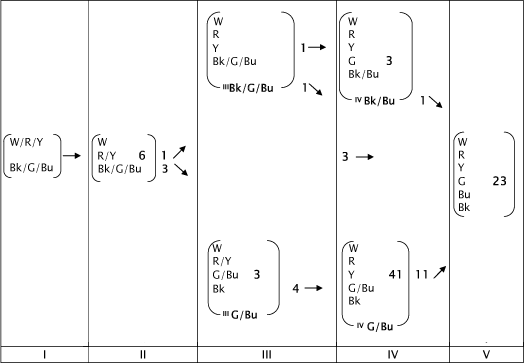
\includegraphics[width=4in]{Graphic/Pictures/fig1.png}
 % fig1.png: 524x363 pixel, 72dpi, 18.49x12.81 cm, bb=0 0 524 363
\end{center}
\caption[A typological and evolutionary scheme]{A typological and
evolutionary
scheme covering most world color survey languages (Source: \cite{Kay99}, Figure
3.)\label{fig:COL-Kay-Maffi-99}}
\end{figure}


The  ancient basics {\S bummo} `black', {\S sɪama} `red'  and    {\S
pʊmma} `white'  are  confirmed at stage
II, a stage where a language has three basic color terms partitioning the
color space. The symbol W stands
for `white' or  `light', the composite symbol R/Y for  `red',  `warm' or 
`yellow',  and  the composite symbol Bk/G/Bu stands for 
  `black' or `dark'. At this
point, if Assumptions 2 is
postulated, we can draw
the conclusion that Chakali is at stage II of the basic color term
typology, as revised and reviewed in,  among others,  \cite{Kay75, Kay97, Kay99,
Kay05}.  According to Assumption 1, the type {IV}_{G/Bu} of stage IV, in
which W  `white', R `red', Y
`yellow', Bk `black' and a composite G/Bu `grue' are the five color partitions,
must be  assigned as it 
fits the characteristics accumulated so far.  This
stage assumes, if 
transitions are treated as successive,  that  the current state derives
from  a  stage where a term to describe either
R/Y  or Bk/G/Bu  existed. Consequently, unless there is 
evidence 
suggesting that  {\S sʊsaʊ} came about as a basic color term before  {\S buluu},
or vice versa, there is no way to know which stage preceded the current one.
The evolutionary schemata of \cite{Kay99}  predicts that Chakali will
partition G/Bu
`grue' in its next stage, i.e.  basic color terms for green and
blue may emerge.






%As \citeauthor{Nade05} writes ``I would strongly suspect that for many English
%speakers their folk-linguistic perception would assume that the fruit is
%called 
%'orange'  because of its colour''\cite[177]{Nade05}.

\section{Usage of color terms}
\label{sec:COL-usage}

Widespread in many societies is the use of color terms in folk
categorization in domains like  zoology, botany, anthropology, etc.
Table 
\ref{tab:COL-usage-color-term} presents various expressions in which color
terms are building blocks. The majority of the expressions  are
qualitative modification in complex-stem noun frames, i.e.  [{\it
stem}$_{1}$]-[{\sc
color}$_{2}$]_{N},  as described in section \ref{sec:GRM-com-stem-noun}.  The
color
term occupies the position of a qualifier, always following the element
qualified. Overall, the meaning of each expression displays different degrees of
opacity, so each of them should be treated  based on its compositional 
transparency. For instance, while {\S nɪ̀búbúmmò}  refers to a
naturally black-brown skinned person,  {\S  pàtʃɪ̀gɪ̀búmmò} does not refer to
a black stomach  but to a non-truthful and non-transparent person, i.e. a liar.
It is not difficult while going down the list of table 
\ref{tab:COL-usage-color-term}  to see that the signification of an expression
is sometimes more precise than, or completely diverges from,  the meaning of its
parts.\footnote{In table \ref{tab:COL-usage-color-term}, a symbol `X' means
that the stem in that position has no meaning on its own, at least
synchronically. There is a consensus among my consultants that the different
types of soil are {\F tʃúr̀} `clay', {\F hàɣlɪ́búmmò} `loamy soil' and {\F
hàɣlɪ́tʃaa} `sandy soil'. In table \ref{tab:COL-usage-color-term},  the
expression {\F hàɣlɪ́sɪ̀ámá}  refers to the kind of soil one can find outside
Chakali land further south, whereas 
{\F hàɣlɪ́pʊ́mmà}  characterises the soil found north of Ducie towards Katua. 
 The expression {\F hàɣlɪ́búmmò} is often associates with the soil found
south of Ducie towards the Mole National Park.  The stem {\F koŋkoɣule} in
{\F kóŋkóɣùlépʊ̀mmá}  `type of egret' has no meaning on its own.} The
expressions in table \ref{tab:COL-usage-color-term} are extracted from the
Chakali
lexicon included in chapter \ref{sec:LEX-lexicon}. It is clear from this short
exposition that it is the trio  {\S bummo}, {\S sɪama} and  {\S pʊmma} which
participates in qualification in complex-stem nouns and helps in
partitioning folk  taxonomies. The same role is not played
by  {\S sʊsaʊ} and {\S buluu}.\footnote{Or any other color term for that matter.
One
exception is   {\F  sànsàndùgúlííhɔ́hɔ́là}  `type of
caterpillar'.}




\clearpage


%\clearpage
% Nevertheless, 
% clayey soil, loamy soil and sandy soil are found at different locations in
%each
% of the
% respective geographical areas. 

\begin{center}

\tablefirsthead{%
\Hline}
\tablehead{%
\hline
\multicolumn{2}{l}{\textit{continued from previous page}}\\
\hline \\[1ex] \hline
}
\tabletail{
\hline
\multicolumn{2}{r}{\textit{continued on next page}}\\
\hline}
\tablelasttail{\Hline}
\topcaption{Color terms in complex-stem nouns 
\label{tab:COL-usage-color-term}}
 
\xentrystretch{0.25} 

\begin{xtabular}{lp{8cm}}

\multicolumn{2}{l}{\it Botany:}\\[1ex] \hline
{\Q kpõ̀ŋkpõ̀ŋsɪ̀àmá} & ({\it lit.}  cassava-red) red
cassava\\
{\Q  kpõ̀ŋkpõ̀ŋbúmmò} & ({\it lit.}   cassava-black) black cassava\\
{\Q  pààtʃákbúmmò} & ({\it lit.}   leaf-black) black leaf or fresh leaf\\
{\Q lúlíbúmmò} & ({\it lit.}   medicine-black) local medicine, such as plant
and tree
products concoction\\
{\Q sɪ̀gpʊ̀mmá} & ({\it lit.}   bean-white) white bean\\
{\Q sɪ̀gsɪ̀àmá} & ({\it lit.}   bean-red) red bean\\
{\Q sɪ̀gbúmmò} & ({\it lit.}   bean-black)  black bean\\
{\Q sɔ̀búmmò}  & ({\it lit.}   thorn-black) Black thorn. {\it Acacia
gourmaensis} \\
{\Q sɔ̀pʊ̀mmá} & ({\it lit.}  thorn-white) White thorn. {\it Acacia dudgeoni}
\\
{\Q sɔ̀sɪ̀ámá} & ({\it lit.}   thorn-red) Red thorn. {\it Acacia hockii} \\
{\Q  nɪ̀ɪ̀pʊ̀mmá} & ({\it lit.}  water-white) liquid coming out of a swelling
which
is operated on  or sap  of a
tree\\
{\Q sɪ̀ŋpʊ̀mmá}& ({\it lit.}    alcoholic.drink-white) palm wine,  made from the
{\it Borassus aethiopum} palm \\
{\Q sɪ́nsɪ̀àmá} & ({\it lit.}   alcoholic.drink-red)  fermented local
brewed drink made from guinea corn, known nation-wide as {\Q pito}\\
{\Q dààsɪ̀àmá} & ({\it lit.}   tree-red) type of tree ({\Q loŋgburɛɛ} in
Waali)\\
{\Q mɪ̃́sɪ̀àmá} & ({\it lit.}   guinea.corn-red) type of guinea corn\\[1ex]
\hline
\multicolumn{2}{l}{\it Zoology:}\\[1ex] \hline
{\Q pèsɪ̀ámá} & ({\it lit.}   sheep-red) red sheep\\
{\Q pèbúmmò} & ({\it lit.}   sheep-black) black sheep\\
{\Q pèpʊ́mmà} & ({\it lit.}   sheep-white) white sheep\\
{\Q nɔ̃̀sɪ̀ámá} & ({\it lit.}   cow-red) red cow\\
{\Q nɔ̃̀búmmò}& ({\it lit.}   cow-black)  black cow\\

{\Q nɔ̃̀pʊ́mmà} & ({\it lit.}   cow-white) white cow\\
{\Q tɛ̀sɪ̀àmá} & ({\it lit.}   X-red) red-flanked duiker. {\it Cephalophus
rufilatus}\\
{\Q dʊ̀ŋmɛ́búmmò}& ({\it lit.}  snake.type-black)
 type of Green-lined snake.  {\it Hapsidophrys lineata}\\
{\Q dʊ̀ŋmɛ́sɪ̀ámà}& ({\it lit. }   snake.type-red)
 type of Green-lined snake. {\it Hapsidophrys lineata}\\
{\Q sànsàndùgúlííbúmmò} & ({\it lit.}  caterpillar-black) type of
caterpillar\\
{\Q  sànsàndùgúlííhɔ́hɔ́là}& ({\it lit.}   caterpillar-{\sc color})  type
of caterpillar\\
{\Q gógósɪ̀àmá} & ({\it lit.}   ant-red) type of ants (Motigu)  {\Q 
haglɪbisɪansa}  (Ducie) \\
{\Q gbɪ̃̀ã̀sɪ̀àmá}& ({\it lit.}   monkey-red) red patas monkey. {\it
Erythrocebus patas}\\
{\Q tʃɪ̃̀ã̀sbúmmò} & ({\it lit.}  fly-black) big black fly which feeds
feeding on carcasses\\
{\Q tʃɪ̃̀ã̀sɪ̀àmá} & ({\it lit.}   fly-red) small red fly usually found with
domestic
animals\\
{\Q kóŋkóɣùlépʊ̀mmá}& ({\it lit.}   X-white)  egret, bird which follows
cows and feeds on the insects which suck their
blood.   {\it Egretta}  \\[1ex] \hline
\multicolumn{2}{l}{\it Farm work and season:} \\[1ex] \hline
{\Q dʒɛ̀fɛ̀búmmò} & ({\it lit.}  farm.state-black)
farm land with a considerable amount of
moisture in the soil\\
{\Q dʒɛ̀fɛ̀pʊ̀mmá} & ({\it lit.}   farm.state-white)
dry farm land, or land with little moisture in
the soil\\
{\Q hàɣlɪ́búmmò} & ({\it lit.}  earth-black)  loamy soil\\
{\Q hàɣlɪ́sɪ̀ámá}  & ({\it lit.}  earth-red)  type of soil\\
{\Q hàɣlɪ́pʊ́mmà}  & ({\it lit.}  earth-white)  sandy soil\\
{\Q tɔ́tʃáámbúmmò}  & ({\it lit.} season.type-black)  transition period
from September
to mid-October, when the fully matured,
thick grasses in the bush begin to diminish
in density\\
{\Q tɔ́tʃááŋsɪ̀àmá}  & ({\it lit.} season.type-red)  transition
period spanning from
mid-October to November, when the rain reduces
drastically and the grasses turn yellow. After this
period comes harmattan.\\[1ex] \hline
\multicolumn{2}{l}{\it Human characteristics:}\\[1ex] \hline
{\Q nɪ̀búbúmmò} &    ({\it lit.}  person-black)
naturally black-brown skinned person\\
{\Q  nɪ̀búpʊ́mmà} &    ({\it lit.} person-white)
naturally white person\\
{\Q nɪ̀búsɪ̀ámá} &  ({\it lit.} person-red) a person with reddish skinned,
atypical
black-brown skin color\\
{\Q  pàtʃɪ̀gɪ̀búmmò} &  ({\it lit.} stomach-black)  a person who is not
truthful, not
transparent, liar\\
{\Q pàtʃɪ̀gɪ́pʊ̀mmá} & ({\it lit.} stomach-white) a generous or fair person\\
{\Q nʊ̀ã̀pʊ̀mmá} &   ({\it lit.} mouth-white) unreserved person, someone
who
cannot keep secrets, who cannot
hold back\\
{\Q sísɪ́àmà} & ({\it lit.} eye-red) seriousness\\[1ex] \hline
\multicolumn{2}{l}{\it Others:}\\[1ex] \hline
{\Q víísɪ̀àmá} &   ({\it lit.} pot-red)  type of water container made out
of clay\\
\end{xtabular}

\end{center}




% 
% We only have two sections in Motigu,
%  Wusiliala
% Wusikuolo
% We have nothing like Wasisiile.
% The inner peel of red cassava is red whilst that of white cassava is white.
% Also, I think white cassava contains some chemicals that can result in stomach
% pains if consumed directly. So often, it is soaked in water for a number of
%days
% to dilute the chemicals. The white is the bitter one.
% Pachegibummo can mean either black leaves or fresh leaves. I think Chakalii
%has
% limited vocabulary so we don't have a clear name for green and blue
% Miisiama is red guinea corn.



\section{Conclusion}
\label{sec:conclusion}

The method used to gather the color terms in Chakali was deficient compared to
the state of the art. The tiles ROR-hue, -T3 and -S3 were destroyed at the
field. This constitutes a  drawback for comparative work. In addition, the 
experiment performed the main task of gathering expressions, a stage of an
experiment called the naming task.  The  focal task was also carried out, but it
was conducted in Wa with only 6 women speakers.  The list task  was not
 carried out.

Although deficient, the method has contributed many  linguistic
expressions  which were subsequently analyzed.  There are in those expressions
interesting linguistic material and research questions (e.g. the role of
reduplication, loans and name-an-object as a first step in designating  `new'
colors, the
problem of ideophones and their foci,  etc.) and socio-linguistic questions
(e.g.  no Waali or Dagaare borrowing). 
Chakali can provisionally be assigned to Stage II  or Stage IV$_{G/Bu}$ of 
\citeauthor{Kay99}'s
system  (see figure \ref{fig:COL-Kay-Maffi-99}),
depending on
the status of the expressions {\S sʊsaʊ} and {\S buluu}. Notice that if we
consider Assumption 1 as correct,  none of the types of the original
typology accomodates the current state of Chakali (see figure
\ref{fig:berlkay3}). 


The relations between (i) a  proportion of the  sample of speakers and a term,
and (ii) a term and a region in the color space were discussed
under the notion of consistency and codability.  We are now in a position to
inspect the Assumptions 1 and 2 of section \ref{sec:prel}. One option is to
treat the terms  {\S sʊsaʊ} and {\S buluu} as basic color terms, the other to
assume  that they are not, but are in a `statistical
transitional'
stage
entering the set of basic color terms, as they are the most codable terms
after the core three. The `basicness' status was measured by establishing that 
a significant proportion of speakers  used a  term to refer to a particular
region of
the color space.

Finally,  if  I eventually decide to carry on with research on Chakali
color terms, the focal task should be carried out with more speakers using all
the consistent terms of the tile naming task. With the focal task
I could find out  the foci of the expressions, and whether some expressions 
lack a foci. The focal task is also crucial in dealing with a
borrowed term like {\S buluu} and a non-consistent term like {\S hɔlahɔla}. Some
results are available for the latter, while the focus of the former is still
unknown. The list task could be carried out as well, although for the
list task to be achieved in a monolingual setting, one needs to design
instructions without a word for `color'.

One remaining question is how `lexicalized' and how `made up' case by case are
the ideophones. Both the tile naming task and the focal task confirmed that
there is an institutionalized repertoire, but  its members are not
associated with  particular color regions, at least I was unable to identify
such   regions with two  methods. Needless to say, this topic deserves further
attention.
